\chapter{Digression - The exact analogy between ultrasound measured acoustics and electromagnetism}\label{ch:interactions}

%\newcommand{\Tgi}{T_{\textrm{gi}}}
%\newcommand{\OmegaEM}{\Omega_{\textrm{EM}}}

 %\newcommand{\tm}{\tau^-}
 %\newcommand{\tp}{\tau^+}

 % \newcommand{\vx}{\vect{x}}
%  \newcommand{\vf}{\vect{f}}
%  \newcommand{\J}{{\cal J}}
% \newcommand{\vJ}{\vect J}
 % \newcommand{\vj}{\vect j}
%  \newcommand{\vE}{\vect E}
%  \newcommand{\vB}{\vect B}
% \newcommand{\vEnr}{\vect{E}_{\textrm{nr}}}
% \newcommand{\vBnr}{\vect{B}_{\textrm{nr}}}
% \newcommand{\va}{\vect a}
% \renewcommand{\vA}{\vect A}
% \newcommand{\jp}{\pi}
% \renewcommand{\M}{\alpha}
% \newcommand{\vP}{\vect P}
%\newcommand{\vf}{\vect f}
% \newcommand{\vF}{\vect F}
% \renewcommand{\AA}{\mathbbm{A}}

% \newcommand{\Dt}{D_t}
% \newcommand{\fbar}{\underline{f}}
% \newcommand{\adjoint}[1]{\bar{#1}}
% \newcommand{\fadj}{\adjoint{f}}

% \newcommand{\zitter}{zitterbewegung}
%\begin{abstract}
%An exact acoustic analogy of electromagnetism is derived
%from a relativistic, isentropic, ideal fluid where the speed of sound is 
%set equal to the speed of light.
%Sound waves and acoustic sources in such a fluid are described by Maxwell's equations.
%It is argued that this is the correct formulation of acoustics 
%when measurements are made with a sonar based technique such as ultrasound.
%\end{abstract}


\section{Introduction}

In \chapref{measurement} we argued that ultrasound is a relativistic theory,
where the sound speed takes the role of the speed of light.
This was argued in terms of the  ultrasound measurement process,
that a constant sound speed must be known before anything can be said about distance.
We also assumed  physical invariance between inertial observers
on the belief that ultrasound should not change this.

Acoustics was then formulated for  a ideal and isentropic fluid.
Consistency with the measurement process required the fluid to be relativistic, 
in the sense that is invariant to Lorentz transformations.
To enforce the sound speed to take the role of the speed of light, 
these two constants were equated.
By enforcing the conservation of the energy momentum tensor
(or equivalently, by Noether's theorem, translational invariance)
we found the temporal and spatial equations of motion,
\eqa{
  \del \cdot A  =0 \tag{\ref{eqn:eomTime}}
}
and
\begin{align}
v \cdot \lr{\del \wedge A} = 0, \tag{\ref{eqn:eomSpace}}
\end{align}
respectively,
where c.g.s. units have been  used.
%From this latter condition a to a conserved energy momentum tensor yields
%
%This latter condition yielded the equation of state $p = \epsilon$,
%where $p$ is the thermodynamic pressure and $\epsilon$ is the total energy density.
%Our starting point was the  conservation of the energy momentum tensor,
%which by Noether's theorem is equivalent to demanding translational invariance.
%
From \eqnref{eomTime} we found that it follows that sound waves and acoustic sources are described by Maxwell's relation,
\eqa{
\del F = J, \tag{\ref{eqn:Maxwell}}
}
where 
\eqa{
  F = \del \wedge A\tag{\ref{eqn:DefnVorticity}}
} is the spacetime vortiticy,
and $J$ is the acoustic source in the wave equation $\del^2 A = J$.
The potential $A \equiv 2\sqrt p v$, where $v$ is the velocity of a fluid particle.

The consequences of this correspondence were not explored, however,
and we tie this loose end here.
In \secref{int:EM} and find that 
the role of magnetism is played by the spatial vorticity of the fluid,
and that the electric field corresponds to the Coriolis acceleration.
The space-time vorticity tensor assumes the role of the electromagnetic field tensor.
This completes similar but partial  attempts by others to construct an analogy between acoustics and electromagnetism.
In particular, both Marmanis\cite{Marmanis2000} and Srihar\cite{Sridhar1998}
have suggested and analogy between vorticity and magnetism, 
and the Coriolis acceleration (or Lamb vector) with the electric field.
However, both authors constructed their analogy in the incompressible Galilean frame, 
and therefore could not write down a wave equation (Maxwell's relation).

% For dimensional consistency we find that the acoustic charge must be {\em dimensionless}.
% The analogue to the electric permittivity has dimension $\joule^{-1}\metre^{-1}$.
% We do not have a satisfactory interpretation for the permitivity, however.

% The formal exactness of the analogy presented here implies
% that the Lagrangian for acoustics (as measured with ultrasound)
% is the same form as the electromagnetic Lagrangian.
% In \secref{int:spin} this fact is used with the further assumption of rotational invariance,
% which  by Noether's theorem demands that angular momentum is conserved,
% to show that an acoustically measured sound wave -just as light- has an intrinsic spin.

The equivalence between electromagnetism and acoustics (as measured with ultrasound)
poses several issues of interpretation:
\nlist{
  \item On the one hand sound is a longitudinal wave, the molecules vibrate parallel to the  perturbation. 
    On the other hand, sound is transverse in the Coriolis acceleration and vorticity.
    In what sense are these two views consistent?
  \item Non-linear propagation is known to be important in ultrasound,
    however, in our formulation it is impossible.
    How can this be.
%  \item Rotational invariance implies that sound has an intrinsic angular momentum.
%    Since there are two possible polarisation of the  Coriolis acceleration and vorticity
%    the sound must be spin 1.
%    What does this mean in terms of the dynamics of the fluid particles?
}
Solutions to both these problems are suggested in \secref{Interpretations}.


%interpretations to these are provided in \secref{FutureWork}.
%There is a speculative nature to these interpretations, however,
%which is why they are considered as future work.
%The difficulties in interpretation come not from dought in the validity

%In \secref{int:spin} we impose rotational invariance,
% the consequences of the correspondence between electromagnetism and acoustics.
%For instance it follows immediately  that sound, when measured acoustically,
%can be considered as transverse wave with respect to  the vorticity and Coriolis acceleration.
%If we further assume of rotational invariance, 
%which by Noether's theorem demands that angular momentum is conserved,
%then we find that sound - just as light - has an intrinsic spin.


% An interpretation of the acoustic spin is provided from the helicity.
% The acoustic analogue to the electromagnetic helicity is identical to the hydrodynamic  helicity introduced by Moffatt.
% It is s a topological invariant that describes the linking between vortex rings,
% and is, therefore, quantised.
% The spin of the sound wave describes the propagation of this topological feature through the medium.

% With these results in hand we consider acoustic-vortex interactions in \secref{int:vortex_interactions},
% important when sound interacts with a region of turbulence.
% When the spin plays no role (unlinked vortices in the turbulence) 
% we find that the interactions are described
% by Lorentz force law.
% This linear relation is a very simple and elegant solution to a difficult problem.
% It also highlights the general rule that the  acoustic measurement greatly simplifies the measured physics.
% This is because acoustic measurement intrinsically limits what can be known about the world.

% The exact analogy suggests that there might be an acoustic analogue to the electron: 
% a particle with helicity that interacts with the spin of the acoustic field.
% We do not succeed in finding the analogue, 
% but a start is suggested in \secref{int:electron}.






 

%Sir James Lighthill, in his formulation of acoustics \cite{Lighthill1952},
%gave a general framework for calculating the sound generated by turbulence with a minimum of approximation.


%The influence of boundaries was added to the formulation by Curle \cite{Curle1955} and Ffowcs Williams and Hawkings \cite{FfowcsWilliams1969}.
%More recently,  formulations in terms of the vorticity and enthalpy have also proven useful \cite{Howe1998}.
%Development has been rapid, and this must be due, in no small part, to the common point of departure enabled by Lighthill.
%The relation of special cases to the whole is clear, it is easy to see the wood from the trees.
% The turbulent sources in Lighthill's theory will in general interact with each other.
% There is a long history in studying the interactions of vorticies \cite{Whittaker1951}, 
% but yet no 
% where the force between the rings `acts at a distance', and  propagates through the medium via sound waves.
% The vorticity formulation of Lighthill's equation, therefore,
% seems ideally placed to formulate sound-acoustic source dynamics in a general way.
% This is a difficult problem in general,
% but a simple solution is possible when the interaction is measured by ultrasound,
% and is outlined in \secref{Lorentz}.
% It turns out that ultrasound is simpler than acoustics in general due to the way in which ultrasound defines time and space.
% This is discussed more in \secref{Measurement}.

% In medical ultrasound, however, the interaction of purely turbulent sources of sound are not of primary interest.
% Rather, focus is directed at the  interactions between  micron-sized pulsating bubbles that are used as contrast agents.
% Usually, when modelling such interactions the fluid is linearised early \cite{Crum1974,Leighton1990, Mettin1997},
% and so any effect of vorticity and turbulence is ignored$rho.
% This is unsatisfactory for two reasons.
% \nlist{
% \item Although the pulsating bubble is likely to dominate the sound generated in a region of turbulence,
%   it does not necessarily follow that the {\em motion } of the bubble is independent of the vorticity in the surrounding fluid.
% \item By linearising the fluid the general framework for sound-acoustic source interactions is being abandoned.
% }
% The first of these problems is the greater when it comes to predicating the results of an experiment.
% However, the second is the more grave.
% By approximating too early the theory becomes separated from the general theory of sound-source interaction, and progress becomes slow.
% Indeed, the Bjerknes force law that is often used to describe the interactions of bubbles has changed little since it was written down in 1905 \cite{Bjerknes1905},
% and this is not because it is without  problems.

% In this report we attempt to bring the description of the motion of a bubble within the Lighthill framework for ultrasonics outlined in \secref{Lorentz}.
% This is attempted in \secref{Zitter}.






\section{The acoustic analogues to the electric and magnetic fields}\label{sec:int:EM}

In classical electromagnetism the electric and magnetic fields are 
3-dimensional vector fields that are measured (usually) in the laboratory frame.
Such spatial vector quantities we denote in bold.
%The laboratory frame is represented by an inertial and orthonormal frame with basis vectors $\{\gamma_\mu| \mu = 0,1,2,3\}$,
%where $\gamma_0$ is a timelike vector with positive signature ($\g^2 =1$) 
%and $\{\gamma_k | k=1,2,3\}$ are spacelike with negative signature ($\g^2=-1$).

The most direct method of obtaining the analogues  is to project the vorticity bivector, $F$, into the laboratory  frame\cite{Hestenes2003, Doran2003}.
The analogue to the electric field can then be defined to be the timelike component, and the analogue to the magnetic field the spacelike component.
The directness of this method, however, comes at the cost of it bearing little  resemblance to conventional acoustics.

To demonstrate the similarities and the differences of ultrasound formulation of acoustics  to the Gallilean formulation,
we re-derive Maxwell's relation using an argument very similar to Lighthill's acoustic analogy\cite{Lighthill1952} of aeroacoustics.
The analogues to the electric and magnetic field  become clear in this process.

We start  by projecting the temporal and spatial equations of motion, equations \eqnref{eomTime} and \eqnref{eomSpace}
into the laboratory frame.
The result is
\sub{
  \begin{align}
     \vdel \cdot \vA &=  - \dt \phi, \label{eqn:Rcontinuity}\\ % &\quad\text{and} &&
\dt \vA - \vv \times  \lr{\vdel \times \vA} \label{eqn:REuler}
&= - \vdel \phi.
  \end{align}
}
$\phi$ and $\vA$ are the temporal and spatial components of the vector potential $A$.
%\eqa{
%\phi &\equiv  \gamma \lr{c^2 + w}  \\ %= A \cdot \g,\gamma \frac{\epsilon + p}{\rho} 2\gamma  p^{1/2}
%& \quad\text{and} &&
%\vA &\equiv  \phi \vv,  %A \wedge \g.
%}
As we found in \secref{measurement:alterations}, $\phi$ may be interpreted as the total enthalpy density,
and $\vA = \phi \vv$.
$\vv$ is the three dimensional velocity.

%Equation \eqnref{continuity} is the ultrasound equiv
Equations \eqnref{Rcontinuity} and \eqnref{REuler} are the acoustically measured versions of the continuity and Euler equations.
In the non-relativistic limit the equations reduce to Galilean invariant forms, 
\sub{
\begin{align}
  \vdel\cdot\lr{\rho \vv}  &= -\dt \rho, \label{eqn:NRcontinuity}\\
  \dt \vv - \vv\times \lr{\vdel\times \vv} &= - \vdel \phi,\label{eqn:NREuler}
\end{align}
}
with 
equation \eqnref{NREuler} being Euler's equation written in Crocco's form\cite{Howe1998}.
The difference between the two sets of equations is that the mass density, $\rho$, in the Gallilean forms is
replaced by the total enthalpy density $\phi$. 
Replacing the mass with an energy is typical of Lorentz invariant theories.

With the continuity and Euler equations in hand,
we may now apply the conventional formulations of acoustics.
We proceed with Lighthill's acoustic analogy\cite{Lighthill1952, Howe1998}.

To do so we   differentiate  the continuity equation (equation \eqnref{Rcontinuity}) with respect to time 
and subtract it from the spatial derivative of  Euler's equation (equation \eqnref{REuler}).
A wave equation for the  total enthalpy results
\subl{
\eqa{
   \lr{\vdel^2 - \dt^2}\phi
  & = \vdel \cdot \lr{\vv \times\lr{\vdel \times \vA} } \equiv - \rho_q.
\label{eqn:WavePhi}
  \intertext{Next, a wave equation for $\vA$ is obtained by 
    by differentiating the continuity equation with respect to space 
    and then adding the result to the temporal derivative of Euler's equation,
    }
   \lr{\vdel^2 - \dt^2}\vA 
   &  = - \vdel\times\lr{\vdel \times \vA} - \dt \lr{ \vv \times \lr{\vdel \times \vA}} \equiv -\vJ.
    \label{eqn:WavevA}
  }
}{Waves}
In keeping with Lighthill's analogy we interpret the right hand side of \eqnref{WavePhi} and  \eqnref{WavevA} 
as an acoustic source density, $\rho_q$, and acoustic current density, $\vJ$, 
respectively.
% Notice the nice property that the current is conserved $\vdel\cdot \vJ + \dt \rho_q = 0$.

For comparison, 
had we carried out this procedure with the Gallilean continuity and Euler equation we would have obtained\cite{Howe1998},
\subl{
  \begin{align}
    \lrsquare{  \Dt \lr{\frac{1}{c^2} \Dt} - \frac{1}{\rho}\vdel \cdot \lr{\rho \vdel}}\phi &= -\frac{1}{\rho} \vdel \cdot \lr{\rho \vv \times \lr{\vdel\times \vv}} \label{eqn:WavephiREG}\\
    \lrsquare{  \Dt \lr{\frac{1}{c^2} \Dt} - \frac{1}{\rho}\vdel \cdot \lr{\rho \vdel}}\vv  &= \frac{1}{\rho} \vdel \times \lr{\rho \vdel \times \vv}. \label{eqn:WavevvREG}
  \end{align}
}{WavesREG}
These are Lighthill's equations expressed in terms of enthalpy and vorticity\cite{Howe1998}.
The operator  $\Dt = \dt + \vv \cdot \vdel$.
The left hand side of both equations \eqnref{WavesREG} describe a non-linear wave in homoentropic potential flow \cite{Howe1998}.

Equations \eqnref{WavePhi} and \eqnref{WavevA} can be simplified by introducing
\begin{align}
  \vE &= - \vv \times \lr{ \vdel \times \vA} &\text{and}&&
  \vB &= \vdel \times \vA,
\end{align}
so that
\subl{
\eqa{
   \lr{\vdel^2 - \dt^2}\phi
  & = - \vdel \cdot \vE  \equiv - \rho_q.
\label{eqn:WavePhiMax}
  \intertext{and
    }
   \lr{\vdel^2 - \dt^2}\vA 
   &  = - \vdel\times\vB + \vE \equiv -\vJ.
    \label{eqn:WavevAMax}
  }
}{WavesMax}
Equations \eqnref{WavesMax} can now be recognised as Maxwell's equations written in terms of the potentials in the Lorenz gauge\cite{Doran2003}.
The vector $\vE$ is the Coriolis acceleration, and takes the role of the electric field in the analogy.
The axial vector $\vB$ is the spatial vorticity and takes the role of the magnetic field.

Writing out Maxwell's 4 equations explicitly gives
\sub{
\eqa{
 \vdel \cdot \vE &= q,\label{eqn:M1}  \\ 
 \vdel \times \vB &= \vJ + \dt E, \label{eqn:M2}\\
 \vdel \times \vE &= -\dt\vB\label{eqn:M3},\\
 \vdel \cdot \vB &= 0\label{eqn:M4},
}
}
The acoustic interpretation of these equations are as follows:
\nlist{
\item Equation \eqnref{M1} is the definition of an acoustic source.
\item Equation \eqnref{M2} is the definition of the acoustic current.
\item Equation \eqnref{M3} is the Lorentz invariant version of the vorticity equation.
\item Equation \eqnref{M4} is an expression of Helmholtz theorem, which demands the conservation of vorticity.
}

%Equations  \eqnref{Waves} are linear, as expected.
%However, it must be emphasised that the lack of non-linearity in \eqnref{Waves} 
%is not due to approximation -  
%equations \eqnref{Waves} and \eqnref{WavesREG} are equally exact.
%Ultrasound acoustics is simpler because less can be 
%known about the medium when it is measured acoustically.

%forms,where $\rho$ is the mass
%It is worthwhile here making a direct comparison.




% The 
% so that
% \eqa{
%  F = F\g\g = \lr{F\cdot\g}\g + \lr{F\wedge \g}\g.
% }
% The analogue to the electric field, $\vE$, and magnetic field, $\vB$,
% %In keeping with convensional formulations of classical electromagnetism,
% %we define the analogues to the electric field, $\vE$, and magnetic field, $\vB$,
% can then be defined \cite{Hestenes, Doran2003} to be 
% \sub{ 
% \label{eqn:DefnEB}
% \eqa{
%   \vE &\equiv  \lr{F\cdot\g}\g = \frac{1}{2}\lr{ F- \g F \g  } = -\dt \vA - \vdel \phi\label{eqn:DefnE}\\
%   \intertext{and}
%   I\vB  &\equiv  \lr{F\wedge\g}\g =  \frac{1}{2}\lr{ F+ \g F \g } = \vdel \wedge \vA,\label{eqn:DefnB}
% }
% }
% respectively.
% Here  $\phi = 2\gamma\sqrt{p}$
% and $\vA = \phi \vv$ are the temporal and spacial components of $A$,
% $\gamma = (1-\vv^2)^{-1/2}$ is the Lorentz  factor and $\vv$ is the spatial velocity vector.
% The term $I$ in \eqnref{DefnB} represents the spacetime pseudoscalar,
% or the `unit volume element' of spacetime.

% To find the rightmost side of \eqnref{DefnE} and \eqnref{DefnB} equation \eqnref{DefnVorticity} has been used,
% and the vector identity $a \cdot \lr{d B} = a\wedge B + d a\wedge B$ for vectors $a$ and $d$, and multivector $B$, is helpful for  \eqnref{DefnB}.
% The spacetime vorticity then exhibits the same `complex' structure as the electromagnetic field tensor,
% \eqal{
% F = \vE + I\vB,
% }{FSplit}
% where the volume $I$ takes the role of the complex number%]
% \footnote{
%   Note that $I^2= \gamma_0\gamma_1\gamma_2\gamma_3 \gamma_0\gamma_1\gamma_2\gamma_3 = -1$.
%   This geometric interpretation of complex numbers is typical of geometric algebra,
%   and gives the algebra huge power\cite{imaginary_numbers_are_not_real}.
% }.

% Expressing \eqnref{DefnB} in terms of the convensional Gibbs vector cross product, denoted with a $\times$,
% we find that $\vB = -I \vdel \wedge \vA \equiv \vdel \times \vA$, 
% and so that the axial vorticity vector is the analogue to the magnetic field.

% An alternative expression for the analogue to the electric field can be found by using equation \eqnref{FSplit} 
% in the orthogonality condition for the velocity and vorticitiy (equation \eqnref{eomSpace}).
% By considering only the bivector quantities (specified by the subscript 2 on the angular brackets $\bivector{\cdot}$)
% it is found that
% \eqa{
%   \bivector{ \g v\cdot F} = \half\bivector{\g v F - \g F v} =\gamma \vE - \gamma \vv \cdot \lr{\vdel\wedge\vA} = 0.
% }
% In the calculation it is helpful to note that $I\vB$ commutes with $\g$ and $\vE$ anti-commutes with $\g$,
% as follows from the second equalities in \eqnref{DefnEB}.
% Therefore, 
% \eqa{
%   \vE = \vv \cdot \lr{\vdel \wedge \vA} \equiv - \vv \times \lr{\vdel \times \vA}, \label{eqn:E}
% }
% which is the Coriolis acceleration.
% The second identity is the result writen with the familiar Gibbs vector product.

% %To prove that the two equations \eqnref{vE1} and \eqnref{vE2} are consistent we note that
% %\eqa{
% %\vv \cdot \lr{\vdel \wedge \vA} = \vv \cdot \vdel \vA - \vdel \vv \cdot \vA = \dt \vA - 
% %}

% \subsection{Maxwell's relation in terms of the Coriolis acceleration and the vorticity}

% Taking the spacetime-split of \eqnref{Maxwell} and using
% \eqnref{FSplit}
% we obtain
% \eql{
%   \lr{\dt + \vdel} \lr{\vE + I \vB} = \rho - \vJ
% }{MaxwellSTSplit}
% where
% \eqa{
% q = J \cdot \g \quad\text{and} \quad
% \vJ  = J\wedge \g.
% }
% Separating out the respective scalar, relative vector,
% relative bivector and relative trivector parts of \eqnref{MaxwellSTSplit}  returns  four equations,
% % \eqa{
% %   \vdel \cdot \vE &= \rho,\\
% %   \dt \vE + \vdel\cdot (I\vB)  &= -\vJ,\\
% %   \del\wedge\vE + \dt(I\vB) &= 0,\\
% %   \del\wedge\vB &= 0.
% % }
% % These may be rewritten 
% \sub{
% \eqa{
%  \vdel \cdot \vE &= q,\label{eqn:M1}  \\ 
%  \vdel \wedge \vB &= I\lr{\vJ + c^2\dt E}, \label{eqn:M2}\\
%  \vdel \wedge \vE &= -\dt(I\vB),\\
%  \vdel \cdot \vB &= 0,
% }
% }
% which are Maxwell Equations written explicitly in terms of the
% acoustic fields.


\subsection{The acoustic sources}
% The acoustic
% From Maxwell's equations we may write explicit forms for the 
% acoustic sources.
% From \eqnref{M1} and \eqnref{E} we have
% \sub{
% \begin{align}
%   q = -\vdel \cdot\lr{ \vv \times \lr{\vdel \times \vA}} \label{eqn:rho}
% \end{align}
% and from equations \eqnref{M2}, \eqnref{E} and \eqnref{DefnB}  we have
% \begin{align}
% \vJ = \vdel \times \lr{\vdel\times \vA} + \dt \lr{ \vv \times \vdel \times \vA}.\label{eqn:vJ}
% \end{align}
% \label{eqn:sources}
% }
% %Note that reintroducing SI units forces the
% %analogue to the electric permittivity to be unity
% %and the analogue to the magnetic permeability to be $c^{-2}$.

% In the non-relativistic limit, equation \eqnref{rho} is 
% the turbulence source term of  Lighthill's formulation of aeroacoustics,
% when written in terms of the total enthalpy and the vorticity\cite{Howe1998}.
% Equation \eqnref{vJ}, however,  seems seldom to be used in the aeroacoustics literature.


It is interesting to note the dimensionality of the acoustic source.
To do so it is necessary to reintroduce SI units so that \eqnref{M1} and \eqnref{M2} become
\sub{
\begin{align}
  \frac{\rho_q}{\epsilon_0} = -\vdel \cdot\lr{ \vv/c \times \lr{\vdel \times \vA}} \label{eqn:rho}
%  \lrsquare{q} = \frac{\text{Energy}}{\text{distance}^2} = \frac{\text{mass}}{\text{time}^2}.
\end{align}
and 
\begin{align}
 \frac{\vJ}{c^2 \epsilon_0} = \vdel \times \lr{\vdel\times \frac{\vA}{c}} + \frac{1}{c^2}\dt \lr{ \vv \times \vdel \times \vA}.\label{eqn:vJ}
\end{align}
}
where $\epsilon_0$ is the acoustic analogue to the electric permittivity.
The units of the left hand side of \eqnref{rho} are
\begin{align}
  \lrsquare{\frac{\rho_q}{\epsilon_0}} = \frac{\text{Energy}}{\text{distance}^2}.
\end{align}
The analogue units in electromagnetism are 
\begin{align}
\lrsquare{\given { \frac{\rho_q}{\epsilon_0}}{\text{em}}} =  \frac{\text{Energy}}{\text{distance}^2\times \text{charge}}.
\end{align}
It follows that the acoustic analogue to charge is {\em dimensionless},
and the analogue to permittivity has the units 
\begin{align}
\lrsquare{\epsilon_0} = \frac{1}{\text{distance}\times\text{Energy}}.
\end{align}
We do not, however, have an adequate interpretation of the acoustic permittivity.
We suppress the issue by  returning to c.g.s. units, where $c= \epsilon_0 = 1$.


%This emphasises what is already obvious from \eqnref{rho},
%that the acoustic charge is a dynamic property of the flow.
%The unit of $\vJ$ is a source term multiplied by a velocity.
%It is consistent with  the current  being a moving charge,
%\begin{align}
%  \vJ = q \vu
%\end{align}
%with $\vu$ being the velocity of the source.

\section{The interpretation of a sound pulse}\label{sec:Interpretations}

The equivalence of the formulation of ultrasound measured acoustics and electromagnetism raises a number of issues of interpretation.
The first of these is the linearity of the theory.
Nonlinear propagation of the sound pulse is well known to be important in ultrasound physics, 
and yet it vanishes altogether in our formulation.
This issue is considered in \secref{NonlinearProp}.

The second is that a sound pulse is a longitudinal wave, the compressions and rarefactions of the density are in the direction of propagation,
whereas Maxwell's relations describe a pair of self interacting transverse waves (the Coriolis acceleration and the vorticity).
The compatibility of these two equations is discussed in \secref{transversivity}

\subsection{On the absence of non-linear propagation} \label{sec:NonlinearProp}

The linearity of the acoustic field is entirely appropriate for ultrasound.
To apply a non-linear wave equation you need to know 
the spatial variations of the speed of sound. 
%which depend in turn, upon the spatial variations of the density.
This is seen in the left hand side of equations \eqnref{WavesREG}.
As argued in \chapref{measurement}, such knowledge is impossible
when using sound to define the concept of distance:
the sound speed used by ultrasound must be a spatially invariant constant to be able to measure anything at all.
What is to be explained, therefore, 
is not why ultrasound measured acoustics is linear - this is surely correct - 
but to explain how the non-linearity found in other measurement systems  manifests itself in acoustic measurements.
To do so it is useful to frame the discussion around the linear acoustically measured equations of
\eqnref{Waves}
and their non-linear Galilean forms \eqnref{WavesREG}.

The first point to note is that the non-linearity of the Galilean formulation of sound is entirely a matter of {\em  convention}.
It would in fact be more appropriate to rewrite equations \eqnref{WavesREG} as linear wave equations with everything else interpreted as acoustic sources and currents.
Then the sound is defined as the part of an acoustic disturbance that can propagate energy away to infinity,
the rest of the disturbance being a `local' source.
This is, in fact, the usual final step of Lighthill's analogy.
The reason it is rarely performed when the analogy is written in terms of the total enthalpy and vorticity is because
the acoustic source terms become horribly complicated.
The split of source and wave in \eqnref{WavesREG} is convenient  interpretatively, but is nevertheless rather ad-hoc,
for it mixes local terms with those that can propagate indefinitely.

The influence of non-linear propagation on what can be measured acoustically is found by comparing the right hand sides of equations \eqnref{Waves} and equations \eqnref{WavesREG}.
It is seen that the only major difference between the two is the term $- \dt \lr{ \vv \times \lr{\vdel \times \vA}}$ on the right-hand-side of \eqnref{WavevA}.
This term is, if you like, the ghost of the non-linear operator $\Dt$ on what can be measured acoustically.
When measured with ultrasound it is interpreted  as part of the current.

We note that an attempt to re-incorporate the ghost  term back into some `acoustically measured non-linear operator' would be ill-conceived, 
for it would mean that the acoustic current is no longer conserved:
the term $- \dt \lr{ \vv \times \lr{\vdel \times \vA}}$ most certainly is a current.






\subsection{Interpreting the transversivity of the sound pulse} \label{sec:transversivity}


An acoustic plain wave is  a  perturbation of the fluid particles in the direction of propagation of the pulse.
It is also a transverse wave in terms of the Coriolis and vorticity fields.
We now propose a method of squaring these seemingly contradictory views.

We consider a segment of the plain wave to be a narrow tube,
so that the entire plain wave is formed by adding together many such tubes.
Within the tube a pertabation in pressure propagates the sound wave longitudinally.
Outside of the tube no such pertabation exists.

Both within and outside of the tube  there is no vorticity and so there is no propagation of the transverse wave.
On the interface of the tube, however, there is shearing of the fluid:
the molecules  within tube move as the wave passes, the molecules outside do not.
This shearing induces a {\em vortex sheet} on the interface \cite{Howe1998}.
The vorticity is confined to the sheet 
and has a strength equal to the average speed of the molecules on either side of the interface.
From the acoustic analogue Maxwell's equations, this vorticity then induces a Coriolis acceleration orthogonal to the interface.
A longitudinal wave therefore  induces a transverse wave on its boundary.

There remains a difficulty with this interpretation, however.
A transverse wave should have exactly two helicity states.
The interpretation given to the first seems, to the author at least, entirely plausible.
The second is more difficult, however.
The construction of a transverse wave with the Coriolis and vorticity vectors interchanged does not seem obvious.
Rather than speculate, 
we leave this question unanswered.



% for the direction of the vortex  difficult, however. , We have given an 
% That is, the vorticity and the 


% Within the perturbation the vorticity vanishes
% and so it is temping to state that $\vB = 0$, innihilating the helicity with it.
% However, this view is not correct.
% To see this we imagine a  wave confined to a narrow tube of radius $r$.
% The plane wave can then be constructed from many  such tubes (see \figref{tubes}).

% At the boundary of an isolated tube slipping occurs between the translating particles that carry the sound
% within the tube
% and the bulk fluid outside.
% This results in a {\em vortex-sheet}\cite{Howe} on the boundary of the tube.
% Also at the boundary there is a discontinuity in the enthalpy $\phi$, 
% carried over from the velocity contribution of $\gamma$ in \eqnref{}.
% The Corriolis acceleration, from  \eqnref{}, therefore has two components.
% A component parallel to the tube $\vE_\parallel$ from the $\dot A$ term and a perpendicular component $\vE_\perp$ from the $\vdel \phi$ term.


% which contains 
% The vorticity from adjacent tubes cancel, 
% but the vorticity at the boundary never does.
% From equation \eqnref{} (Crocco's equation, in the hydrodynamics literature)
% The vorticity on the boundary induces a Coriollis acceleration,
% we see that on the boundary the vorticity 

 
% and it is this sense that a sound pulse can be considered as a transverse Coriollis-voriticity wave.
% The transversivity must can be set in two directions which can be described as being in either a {\em left-}  or {\em right-handed polarisation state},
% and so the helicity must be in one of two states.


% Nevertheless, for the sound pulse not to have a preferred direction, 
% and therefore to conserve angular momentum,
% it is required that it the particle  streamlines form a knot over this infinite interval.
% Perhaps the simplest vortex  knot that may be considered is the trefoil knot illustrated in \figref{}.
% Topologically the trefoil knot is equivalent to two linked rings,
% each  with the same circulation, $\kappa$, as the knot.
% The helicity of the trefoil knot is accordingly $\pm2\kappa^2$.


% The helicity of a photon is $\pm\hbar$.
% If sound is knotted with the simple trefoil knot then the {\em acoustic Plank's constant} would be
% \begin{align}
%   \hbar = 2\kappa^2,
% \end{align}
% (divided by a unit momentum, see footnote \ref{footnote:dimensionallity_footnote}).

% Why $\hbar$ and therefore $\kappa$


% Moffatt's topological interpretation of helicity has been used before to  interpret the quantisation
% of the spin in electrodynamics.
% See, for example the extensive investigations into the {\em magnetic helicity} of Trueba and Ra{\~n}ada\cite{Trueba1996, Trueba2000, Ranada2002}
% (The magnetic helicity is equation \eqnref{Helicity} where the $\vA$ and $\vB$ have there electromagnetic interpretation).
% %This in fact continues the very old notion of the vortex atom
% %that goes back to the very formulation of electrodynamics.
% What is new
% in this thesis is the equivalence of electromagnetic field and the acoustical field.
% The hydrodynamic helicity is the {\em same} as the acoustic helicity;
% the  sound pulse has a quantised spin
% and  this spin may be interpreted, via the  helicity,
% as the orbital angular momentum of  the fluid particles about their mean flow.
% %\cite{Moffatt1969, Moffatt1988, Chechkin1993,  Trueba1996, Trueba2000}.

\section{Discussion}

This  chapter has explicitly formulated the (exact) analogy between ultrasound measured acoustics 
and electromagnetism.
This ties the loose ends of \chapref{measurement}, where the analogy was noticed but not explored.
It has been found that the acoustic analogue to the electric field is the Coriolis acceleration,
and that the acoustic analogue to the magnetic field is the vorticity,
The spacetime vorticity bivector takes the role of the field tensor.
The analogy in this form has long been suspected\cite{Marmanis2000,Sridhar1998},
however, to the authors knowledge this is the first time that the analogy has been  completed.
The key step, missing in previous attempts, 
is to note that acoustics must be formulated in terms of a Lorentz invariant fluid where
{\em the speed of sound equals the speed of light}.
It is only when this step is made that the analogy exists.

Relativistic fluids where the sound speed equals the speed of light have been studied many times before
as theoretical curiosities\cite{Taub1978,Pekeris1977}.
For example, Pekeris observed that Hick's spherical vortex conserves angular momentum if and only if
the sound speed equals the speed of light\cite{Pekeris1977}.
The importance of such fluids, however, has not to the authors knowledge been recognised.
Such fluids represent {\em what can be measured} when distances are obtained by echo-location.
Acoustics as measured with ultrasound is therefore {\em identical} to electromagnetism (as measured with light).
Retrospectively this correspondence is not too surprising.
For both acoustics as measured with ultrasound and electromagnetism as measured with light 
attempt to measure the properties of their propagating signal.
Both, therefore, 
represent a similarly limited view of the world,
the limitations manifesting themselves in the linearity of the equations.

Another interesting analogy between acoustics and electromagnetism is `acoustic analogue gravity' literature (see Barcel{\'o}, Liberati and Visser\cite{Barcelo2005} for a review).
The approach constructs an {\em acoustic} metric that describes the acoustics of sound carried in bulk flow.
While the description of space and time in this formulation is Euclidean, the acoustic metric turns out to be pseudo-Euclidean,
and therefore obeys the Lorentz transformation.
This results because sound carried away in bulk flow  faster than the speed of sound will never reach us.
The speed of sound is  therefore a limiting velocity in transformations.
The analogue gravity literature then goes on to study the gravitational implications of the acoustic metric.

While the motivations behind the two approaches is similar, in particular the demand that acoustics must be obey a Lorentz invariant metric,
the approach given here and the approach of analogue gravity are fundamentally different.
Analogue gravity does not consider the measurement process and so operates within a world characterised by two metrics, 
the Lorentz invariant acoustic metric and the Galilean invariant spacetime  metric.
Ultrasound measurement demands that the world be described by a Lorentz invariant metric.
There is no other way to describe space and time acoustically.
In analogue gravity the acoustic metric is Lorentz-invariant, but is not the same as the metric used here.
In analogue gravity the metric is a function of the bulk flow,
whereas  we argue that this is impossible:
the sound speed must be an a priori constant in order to say anything about the world.
Nevertheless, the success of analogue gravity is very encouraging.
Acoustically observed microbubbles could offer an interesting experimental model in this field.



% The speed of sound is similarly limiting.
% This observation is then used to pursue the 
% The approach  starts by noting that sound carried away by a bulk flow travelling faster than the speed of sound will never reach us.
% In this sense, the acoustic source is silent, and not, perhaps dissimilar to an a
% emitted by an acoustic source that is carried away by bulk flow faster than the speed of sound.Starting from the observation that it is impossible to measure the acoustics of a 

\subsection{The acoustic Lagrangian}\label{sec:int:spin}
Finally, let us use the acoustic analogy to set out some directions for future work.
%%
%
%Usually, when imagining the average motion of particles in a sound wave,
%we think of the particles oscillating back and forth as the pressure perturbation passes through.
%This is because we think of sound waves as being longitudinal.
%In equation \eqnref{Maxwell} we have an exact analogy between electromagnetism and ultrasound measured acoustics.
%that a sound waves can be considered to be a self-inducing vorticity-Coriolis wave.
%The transverse nature (with respect to the direction of propagation)  of electromagnetic waves is well known, and applies equally to the vorticity and Coriolis fields here.
%In this section we consider the implications of this observation.
%\subsection{The acoustic Lagrangian}\label{sec:lagrangian}
%From equations \eqnref{Maxwell} acoustic sources are described by the same equations that characterise electromagnetic sources.
The common mathematical  description between acoustics and electromagnetism can be enforced by deriving both from a Lagrangian of the same form.
The electromagnetic Lagrangian density is\cite{Lasenby1993, Doran2003},
\begin{align}
 \L = \frac{1}{2} F \cdot F  - A \cdot J, \label{eqn:Lagrangian}
\end{align}
and the acoustic Lagrangian is same so long as the symbols $F$, $A$ and $J$ take their 
acoustical meaning.
Note that the acoustical Lagrangian is not the same as the Lagrangian of the ideal fluid.
It describes directly the sound and the acoustic sources,
rather than the fundamental motions of the fluid particles.



%\subsection{Symmetries from the Lagrangian density}
The symmetries of \eqnref{Lagrangian} can be found by minimising the action,
\begin{align}
  S =  \int \abs{d^4x} \L(A, \del\wedge A; x).
\end{align}
In the absence of acoustic sources ($J=0$) this results in the Euler-Lagrange equation 
\begin{align}
  \d_A \L + \del \cdot  \lr{\del_{\del\wedge A}\L} = 0. \label{eqn:EL}
\end{align}
Demanding translational invariance of the action and assuming that the
Euler-Lagrange equations are satisfied results (via Noether's theorem) in the conservation of the acoustic energy momentum tensor\cite{Lasenby1993,Doran2003}  
\eqa{
   T\lr{a} = -\half F a F.
} 
Demanding rotational invariance and applying \eqnref{EL} results in the conservation of the angular momentum.
The adjoint to the angular momentum tensor is the most useful and is\cite{Lasenby1993,Doran2003}  
\begin{align}
 \adjoint{\J}(n) = A \wedge \lr{F\cdot n} +  \adjoint{T}(n) \wedge x.
\end{align}
The second term,  $\adjoint{T}(n) \wedge x$, is the orbital angular momentum of the sound pulse as
moves through space.
The first,
\begin{align}
S(n) = A \wedge \lr{F\cdot n},
\end{align}
is the intrinsic spin of the  acoustic field.

The acoustic energy momentum tensor can be applied immediately to derive the 
 force law for an acoustic source when in the presence of an external vorticity or Coriolis field.
Remembering Maxwell's relation, $\del\cdot F = J$ (equation \eqnref{Maxwell})
we obtain 
\begin{align}
 f = \scope T(\scope \del) = -\half \lr{\scope F\scope \del F + F \del F} = -\half \lr{-JF +FJ} = J \cdot F.
\end{align}
If the acoustic source has a constant rest mass, $m_0$, and moves at a speed $u$,
then, by writing  $J = q u$, where $q$ is the acoustic source, we obtain
\begin{align}
  f = m_0 \dot u = q u \cdot F, \label{eqn:LFL}
\end{align}
Equation \eqnref{LFL}  is the Lorentz force law.

To write equation \eqnref{LFL} in its more conventional form we project into the laboratory frame,
\begin{align}
J\cdot F  = \scalar{\lr{\rho + \vJ} \g\lr{\vE+I\vB}} = -\lr{J\cdot E + q \vE + q \vu\times\vB }\g.
\end{align}
The timelike $q\vu\cdot\vE $ is the work done.
The remaining spatial component is
\begin{align}
   \vf = -q \lr{\vE + \vu \times \vB},
\end{align}
which is the Lorentz force law in its usual form.

Equation \eqnref{LFL} describes how a turbulent source moves 
in the presence of external flows when measured with ultrasound.
It is an incredibly powerful result.
Its use, however, requires individual acoustic sources to be tracked though space.
This is generally beyond the capability of ultrasound,
although this is changing with the increasing availability of 3 dimensional probes.

%Its linearity is an example of the general rule that the world appears more simple
%when it is measured acoustically.
%This is because, due to the limitations on what ultrasound can measure, reassigns the temporal and spatial locations of entities so that 
%the non-linearity in their motion vanishes.

\subsection{Helicity and Spin}

The existence of the intrinsic acoustic spin raises further interpretative issues.
In the absence of satisfactory explanation for these, however, we resist the temptation to speculate.
All we say on the matter is to note that helicity of the sound wave, 
the projection of the spin on the direction of the momentum, 
is identical to the hydro dynamical helicity introduced by Moffatt\cite{Moffatt1969}.
This is interesting because the integral of the hydrodynamic helicity is a topological invariant that measures the degree of knottedness of the flow\cite{Moffatt1969}.

To see this, we introduce the helicity,
\begin{align}
  \H \equiv   \hat \vP \cdot S(\gamma_0) = \hat \vP \cdot \lr{\phi \vE - \vA \times\vE} =  \frac{\abs{\vE}^2}{\abs{\vE\times\vB}}\vA \cdot \vB.
\end{align}
where  $\hat \vP$ is the unit  Poynting vector, 
\begin{align}
 \hat\vP =\frac{\vE \times \vB}{\abs{\vE\times\vB}}.
\end{align}
and $S(\gamma_0)$ is the timelike component of the Spin 
as measured in the laboratory frame,
\begin{align}
 S(\gamma_0) % &=  A \wedge(F\cdot)  \\
 &= \half\bivector{A\g \g \lr{F\g - \g F}}\\
 &= \phi\vE - \vA \times \vE.
\end{align}
For a sound wave
%\begin{align}
$\abs {\vE} = c\abs{\vB}$
%\end{align}
and so the helicity simplifies to
\begin{align}
  \label{eqn:Helicity}
\H = \vA \cdot \vB.
\end{align}

% To interpret the spin it is useful to project it onto the direction of motion,
% yielding a scalar known as the helicity,
% \begin{align}
%   \H = \hat \vP \cdot S(\gamma_0),
% \end{align}
% where  $\hat \vP$ is the unit  Poynting vector, 
% \begin{align}
%  \hat\vP =\frac{\vE \times \vB}{\abs{\vE\times\vB}}.
% \end{align}
% and $S(\gamma_0)$ is the timelike component of the Spin 
% as measured in the laboratory frame,
% \begin{align}
%  S(\gamma_0) % &=  A \wedge(F\cdot)  \\
%  &= \half\bivector{A\g \g \lr{F\g - \g F}}\\
%  &= \phi\vE - \vA \times \vE.
% \end{align}
% The helicity is therefore
% \begin{align}
%   \H =  \hat \vP \cdot \lr{\phi \vE - \vA \times\vE} =  \frac{\abs{\vE}^2}{\abs{\vE\times\vB}}\vA \cdot \vB.
% \end{align}
% For a sound wave
% %\begin{align}
% $\abs {\vE} = c\abs{\vB}$
% %\end{align}
% and so the helicity simplifies to
% \begin{align}
%   \label{eqn:Helicity}
% \H = \vA \cdot \vB.
% \end{align}
% While $\H$ in \eqnref{Helicity} is defined in terms of the spin,
%  the 
 The term $\vA \cdot \vB$ on the right hand side is the same as the 
relativistic generalisation\footnote{ \label{footnote:dimensionallity_footnote}
The relativistic generalisation is accomplished by replacing $\vv$ in Moffatt's definition with $\vA$.
Notice, furthermore, that Moffatt did not normalise the Helicity,
that is $\H_{\text{Moffatt}} = p\cdot S$ rather than $\frac{1}{\abs{p}}p\cdot S$,
where $p$ is the momentum.
When we make the comparison to $\H = \epsilon_0 A\cdot B$, therefore,
we implicitly divide $\H_{\text{Moffatt}}$ by a unit momentum,
so that dimensionally all is correct.
} to the
{\em hydrodynamic helicity} per unit volume defined by Moffatt\cite{Moffatt1969}.
It is also  readily interpretable.
$\vB = \vdel \times \vA$ measures a rotation,
and the rotation is projected about  $\vA$.
The helicity therefore measures the degree to which the fluid streamlines rotate about themselves,
that is, the degree to which the streamlines are helical\cite{Moffatt1969, Ranada1992}.
%In a small volume $dV$ the flow is comprised of a superposition of a uniform flow $A_0$, a shear
%and a rigid body rotation about the origin of $dV$ with an angular velocity of twice the vorticity $2\vB_0$
%The streamlines of the flow within the sound pulse will be helices about the sheared $A_0$
The contribution to $\vA \cdot \vB dV \approx \vA_0\cdot \vB_0 dV$
is positive or negative depending on the orientation of the helix\cite{Moffatt1969}.

In this way Moffatt identifies the component of the spin parallel to the momentum
with the {\em orbital angular momentum} of a fluid streamline about its mean trajectory.
The equivalence between the two helicities (acoustic and hydrodynamic)
suggests that this interpretation of the spin is valid.

Finally we note that the hydrodynamic helicity was introduced by Moffatt because 
\begin{align}
  I = \int \abs{dV} \H = \int \abs{dV} \vA \cdot \vB
\end{align}
is an invariant that defines the degree of knottness of the fluid.
In the case of two vortex rings, for example, $\H =2 \alpha \kappa_1 \kappa_2$ 
where $\kappa_i$ are the circulations around the two rings. % $C_i$ of the two vortex filaments,
%\begin{align}
%  \kappa_i = \oint_{C_i} \vu \cdot d\vect{l},
%\end{align}
%where $\vu$ is the velocity around $C_i$,
%and $\alpha$ is an integer that defines the linking of the two filaments.
If they are unlinked $\alpha = 0$, whereas if they are singularly linked $\alpha = \pm 1$.
The helicity in a volume, the component of the spin parallel to the momentum, is therefore quantised
in accordance with the topology of the streamlines.

The author does not have an interpretation for this fascinating result and so does not comment further.
We note, however, that there has been considerable effort in applying the hydrodynamic helicity electromagnetism,
with implications to both the quantisation of the spin and to the quantisation of the charge.
We refer the interested reader to the literature\cite{Trueba1996, Trueba2000, Ranada2002}.




% that the projection of the spin along the direction of the acoustic momentum,
% We do not wish the resThis is necessary to avoid confusing the results already given 

% in the absence of sources ($J= 0$) by writing $A \rightarrow A + \epsilon \AA$,
% where $A$ is the  minimum field, $\epsilon$ is a small number and $\AA$ is a perturbation about $A$.
% Then 
% \begin{align}
% \frac{d S }{d\epsilon}&= \int \abs{d^4x}\lr{\AA \cdot \d_A \L + (\del\wedge \AA) \cdot \del_{\del\wedge A}\L}\\
% &= \int \abs{d^4x} \int \abs{d^4x} \AA \cdot\lr{ \d_A \L + \del \cdot  \lr{\del_{\del\wedge A}\L} } + \text{b.c}
% \end{align}
% where $\text{b.c}$ indicates the presence of  a total divergence which is assumed to vanish on the boundary.
% When $S$ is minimised,
% \begin{align}
%   \d_A \L + \del \cdot  \lr{\del_{\del\wedge A}\L} = 0, \label{eqn:EL}
% \end{align}
% which is the Euler-Lagrange equation for the acoustic field.
% x\subsubsection{Transformations}
% A transformation in the underlying space 
% \begin{align}
% x \rightarrow x^\prime = f(x)
% \end{align}
% maps one location $x$ in space to another, $\xp$.
% A tangent vector $a(x)$ to the space at $x$ 
% is then mapped to 
% \begin{align}
%    a(x^\prime) = a\cdot \del f(x) \equiv \fbar(a).
% \end{align}
% The adjoint, $\fadj$ to this transformation is defined by the relation
% \begin{align}
%    b^\prime \cdot \fbar(a) = a\cdot \fadj(b^\prime) 
% \end{align}
% so that 
% \begin{align}
% \fadj(b) = \del_a  \fbar(a)\cdot b  = \del f(x) \cdot b.
% \end{align}
% It follows that
% \begin{align}
%   \del a(\xp) &= \del_b b\cdot \del a(f(x))\\
%   %&= \del_b \lr{b\cdot \del f(x)} \cdot \del_{x^\prime} a(x^\prime) \\
%   &= \del_b \fbar(b) \cdot \del_{\xp} a(\xp)\\
%   &= \fadj(\del_\xp) a(\xp).
% \end{align}
% Therefore 
% \begin{align}
%   \del &= \fadj(\del_{x^\prime}) \equiv \fadj(\del^\prime). \label{eqn:delTransformation}
% \end{align}
% All vectors must transform the same way,
% and so more generally we define
% \begin{align}
%   a^\prime(x) = \fadj(a(x^\prime)) = \fadj\fbar(a(x)).
% \end{align}

% % In summary, therefore, the transformation $\xp =  f(x)$
% % induces the transformations
% % \sub{
% % \begin{align}
% %   a(x^\prime) &=  \fbar(a(x)) 
% % \intertext{and }
% %   \del &= \fadj(\del_{x^\prime}) \equiv \fadj(\del^\prime).
% % \end{align}
% % \label{eqn:InducedTransformations}
% % }
% The action transforms under a change of coordinates as 
% \begin{align}
%   S = \int \abs{d^4x} \L(A, \del\wedge A; x) = \int \abs{d^4x^\prime}\det \fbar^{-1} \L(A^\prime, \del^\prime\wedge A^\prime; x^\prime)
% \end{align}
% and so 
% \eqa{
%   \L^\prime(A, \del\wedge A;x) = \frac{1}{\det \fbar} \L(A^\prime, \del^\prime\wedge A^\prime; x^\prime).
% }
% Parameterising the transformation by the scalar $\alpha$,  where $\alpha=0$ corresponds to the identity transformation,
% gives
% \begin{align}
% \given{\frac{d \L^\prime }{d\alpha}}{\alpha=0} &= \delta A^\prime \cdot \del_{A^\prime}\L + \lr{\del^\prime\wedge (\delta A^\prime)}\cdot \del_{\del^\prime\wedge A^\prime} \L
% \end{align}
% where the shorthand $\delta A^\prime = \frac{d A^\prime}{d\alpha}$ has been used.
% If it is assumed that  $A$ satisfies the Euler-Lagrange equation,  \eqnref{EL}, 
% then 
% \begin{align}
%   \given{\frac{d \L^\prime }{d\alpha}}{\alpha=0}  &= \del\cdot\lr{\lr{\delta A^\prime} \cdot \del_{\del^\prime\wedge A^\prime} \L}.
%   \label{eqn:dL}
% \end{align}
% %on the condition that, on the second line,  $A$ satisfies the Euler-Lagrange equation,  \eqnref{EL}.
% %If the Lagrangian density is symmetrical to the transformation the $\L$ is independent of $\alpha$ and 
% %{\em conjuagate current} $\lr{\delta A} \cdot \del_{\del_{x^\prime}\wedge A^\prime} \L$ is conserved.

% \subsection{Translational Invariance}
% If there is no priviliged position in space then the Lagrangian  density should be unchanged by the transformation
% \begin{align}
%   x^\prime = x + \alpha a,
% \end{align}
% for constant vector $a$ and scalar $\alpha$.
% The differential to the transformation is $\fbar(a) = a$
% the adjoint is  $\fadj(a^\prime) = a^\prime$,
% and the determinant is 1.
% Therefore  $A^\prime(x) = A(x)$ and the $\del = \del^\prime$.
% We also have  $\delta A^\prime = a\cdot \del A$
% and  $\frac{d \L(x^\prime }{d\alpha} = a \cdot \del \L(x)$.

% Equation \eqnref{dL} then becomes 
% \begin{align}
%   a\cdot \del \L =  \lr{a\cdot \del A} \cdot \del_F \L = \lr{a\cdot \del A} \cdot F,
% \end{align}
% from which it follows that, 
% \begin{align}
% \del\cdot\lr{\lr{a\cdot \del A} \cdot F - a\L} = 0.
% \end{align}
% The energy-momentum tensor, 
% \begin{align}
%   T(a) = \lr{a\cdot \del A} \cdot F - a\L = \lr{a\cdot \del A} \cdot F -\half a F\cdot F, \label{TEM}
% \end{align}
% is therefore conserved for translations through space-time.

% The explicit dependence on $A$ can be moved to the bounding surface\cite{Lasenby1993,Doran2003}
% by writing  $a\cdot\lr{\del \wedge A} =a \cdot \del A -  \del\lr{ A \cdot a}$
% so that
% \begin{align}
% \label{eqn:TAEM}
%   \Tgi(a) = \lr{a\cdot F}\cdot F  -\half a F\cdot F = - \half F a F
% \end{align}
% plus a total divergence, which is assumed to vanish on the boundary at infinity.
% The energy momentum tensor is then in a  manifestly gauge invariant form within the volume.
% $\Tgi$ is equal to its adjoint $\bar {\Tgi}$
% and so translational symmetry implies that  $\del \cdot \Tgi(a) = a\cdot\scope\Tgi(\scope\del) = 0$.
% This follows because
% \eqa{
%   \bar T(a) &= -\half \del_b \scalar{a F b F} \\
%   &=-\half \del_b \scalar{b F a F} \\
%   &= -\half F a F = T(a).
% }
% \subsection{Acoustic spin from rotational invariance}

% In addition to translational invariance, 
% all physical theories should be invariant to rotations:
% there should be no preferred orientation to our experiments.

% Rotations are represented by the transformation 
% \begin{align}
%   x^\prime = \Rt x R, \label{eqn:RotTrans}
% \end{align}
% where $R = e^{\alpha B/2}$ and $\Rt = e^{-\alpha B/2}$
% each represent rotations by the angle $\alpha/2$ through the plain $B$%
% \footnote{
% If $x$ is in the plain $B$ then, $B$ anti-commutes with $x$
% so that $\Rt x R = x e^{\alpha B}$. 
% Furthermore, if $B$ is composed of normal vectors of the same signature,
% for example $B = \gamma_1\wedge\gamma_2 = \gamma_1\gamma_2$ then
% $B^2= -1$.
% Equation \eqnref{RotTrans} then comprises of a rotation in the `complex plain'  $\gamma_1\gamma_2$.
% For the three spatial rotations there are three such plains and so three such complex numbers.
% These were introduced by Hamilton as $i$, $j$, $k$ in his Quaternian algebra,
% and is where, historically, the index notation comes for the three spacial axes.
% The double sided rotation of $\alpha/2$ degrees alluded Hamilton, however,
% and  this meant that rotations could only be handled if the vector to be rotated was in the same plain as the rotation.
% This made the algebra complicated, 
% and cause Gibbs to break apart Quaternian into the  $i$, $j$, $k$ axes and a scalar.
% For more on this history see the books of David Hestenes\cite{Dynamicsbook, Hestenes1984} and the Cambridge geometric algebra group\cite{Doran2003}.
% }.
% The differential of the transformation is $\fbar(a) = \Rt a R$ 
% the adjoint is $\fadj(a^\prime) = R a \Rt$ and the determinant is unity.
% Using $R\Rt =1 $ it follows that 
% \begin{align}
%   A^\prime(x) = R A(\xp) \Rt = A(x).
% \end{align}
% Using \eqnref{delTransformation} it follows that 
% \begin{align}
%  \del \wedge A = R \del^\prime \wedge A(x^\prime) \Rt = R F(\xp) \Rt.
% \end{align}
% The vector 
% \begin{align}
% \delta A^\prime &= \frac{d}{d\alpha}R A(x^\prime) \Rt \\
% &= B\cdot A + R \frac{d \xp}{d \alpha}\cdot \del A \Rt \\
% &=  B\cdot A - \lr{B \cdot x }\cdot \del A.
% \end{align}

% Using \eqnref{dL} we obtain the conserved current, the angular momentum 
% \begin{align}
%   \J(B) &= \lr{B\cdot A - \lr{B \cdot x }\cdot \del A}\cdot F+ \half B\cdot x F\cdot F\\
%   &= \lr{B\cdot A} \cdot F + T(x\cdot B)
% \end{align}
% where \eqnref{TEM} has been used.
% The adjoint is 
% \begin{align}
%   \adjoint{\J}(n) &= \del_B\scalar{\J(B) n} \\
%   &= \bivector{A F\cdot n - x\wedge \del T(x) \cdot n} \\
%   &= A \wedge \lr{F\cdot n} +  \adjoint{T}(n) \wedge x
% \end{align}
% The second term  $\adjoint{T}(n) \wedge x$ is the orbital angular momentum of the sound pulse as
% moves through space.
% The first
% \begin{align}
% S(n) = A \wedge \lr{F\cdot n}
% \end{align}
% is the intrinsic spin of the  acoustic field.
% The spin term is often suppressed by putting its influence in the boundary conditions,
% but since we are interested in acoustic plain waves we shall not do this.
% %This has the advantage of making the angular momentum manifestly gauge-invariant,
% %although at the cost of making plain-waves (that reach to infinity) more inconvenient to handle.
% %Again this isn't manifestly gauge invariant.
% %When the fields diminish rapidly at infinity the angular momentum may be  expressed in gauge invarent form,
% %the spin is absorbed into the angular momentum $T(n)$.
% %However, such a procedure is not valid for plain wave solutions (as the field does not vanish at infinity)
% % so we keep \eqnref{AM}.
% %The spin in the lab frame  is
% %\begin{align}
% %  S(v) =A \wedge   \lr{F \wedge \gamma} = -\multi{\phi + \vA \vE}_2 = \phi phi I \vB_v 
%  %  S(n) = A \cdot  \lr{F\wedge  n} =  \lr{A\cdot F} \wedge n %= -\phi I\vB
% %\end{align}
% %The spin in the lab frame  is
% %\begin{align}
% %  S(\g) =A \wedge   \lr{F \cdot \g} = -\phi \vE - I \vA \times \vE  = 
% % %  S(n) = A \cdot  \lr{F\wedge  n} =  \lr{A\cdot F} \wedge n %= -\phi I\vB
% %\end{align}

% \subsection{The acoustical spin as a quantised topological invariant}

% To interpret the spin it is useful to project it onto the direction of motion,
% yielding a scalar known as the helicity,
% \begin{align}
%   \H = \hat \vP \cdot S(\gamma_0),
% \end{align}
% where  $\hat \vP$ is the unit  Poynting vector, 
% \begin{align}
%  \hat\vP =\frac{\vE \times \vB}{\abs{\vE\times\vB}}.
% \end{align}
% and $S(\gamma_0)$ is the timelike component of the Spin 
% as measured in the laboratory frame,
% \begin{align}
%  S(\gamma_0) % &=  A \wedge(F\cdot)  \\
%  &= \half\bivector{A\g \g \lr{F\g - \g F}}\\
%  &= \phi\vE - \vA \times \vE.
% \end{align}
% The helicity is therefore
% \begin{align}
%   \H =  \hat \vP \cdot \lr{\phi \vE - \vA \times\vE} =  \frac{\abs{\vE}^2}{\abs{\vE\times\vB}}\vA \cdot \vB.
% \end{align}
% For a sound wave
% %\begin{align}
% $\abs {\vE} = c\abs{\vB}$
% %\end{align}
% and so the helicity simplifies to
% \begin{align}
%   \label{eqn:Helicity}
% \H = \vA \cdot \vB.
% \end{align}
% %On the left is the electromagnetic helicity. 
% %On the right is the acoustical helicity first defined by Moffat \cite{Moffatt1969}.

% %For the acoustic wave to be transverse in vorticity the particles being perturbed must contribute to  an angular momentum (spin) when the sound wave passes through.
% %We must therefore imagine the particles to be moving on small vortex lines, 
% %rather than `to and throw' in a linear fashion.
% %These loops must be closed, for else momentum will be passed to the fluid  after the sound wave has passed,
% %and the the longitudinal oscillation should coincide with the frequency of the wave. 
% %A motion such as the streamline in \figref{particle} could be imagined.



% %The loop drawn in \figref{particle} may seem overly complicated.
% %The reason that a simple circle, for example, 
% %would not do is due to the non-trivial topology implied by the non-vanishing helicity.
% While $\H$ in \eqnref{Helicity} is defined in terms of the spin,
%  the  term $\vA \cdot \vB$ on the right hand side is the same as the 
% relativistic generalisation\footnote{ \label{footnote:dimensionallity_footnote}
% The relativistic generalisation is accomplished by replacing $\vv$ in Moffatt's definition with $\vA$.
% Notice, furthermore, that Moffatt did not normalise the Helicity,
% that is $\H_{\text{Moffatt}} = p\cdot S$ rather than $\frac{1}{\abs{p}}p\cdot S$,
% where $p$ is the momentum.
% When we make the comparison to $\H = \epsilon_0 A\cdot B$, therefore,
% we implicitly divide $\H_{\text{Moffatt}}$ by a unit momentum,
% so that dimensionally all is correct.
% } to the
% {\em hydrodynamic helicity} per unit volume defined by Moffatt\cite{Moffatt1969}.
% It is readily interpretable.
% $\vB = \vdel \times \vA$ is measures a rotation,
% and the axis of rotation is set by $\vA$.
% The helicity therefore measures the degree to which the fluid streamlines rotate about themselves,
% that is, the degree to which the streamlines are helical\cite{Moffatt1969, Ramada1992}.
% %In a small volume $dV$ the flow is comprised of a superposition of a uniform flow $A_0$, a shear
% %and a rigid body rotation about the origin of $dV$ with an angular velocity of twice the vorticity $2\vB_0$
% %The streamlines of the flow within the sound pulse will be helices about the sheared $A_0$
% The contribution to $\vA \cdot \vB dV \approx \vA_0\cdot \vB_0 dV$
% is positive or negative depending on the orientation of the helix\cite{Moffatt1969}.

% In this way Moffatt identifies the component of the spin parallel to the momentum
% with the {\em orbital angular momentum} of a fluid streamline about its mean trajectory.
% The equivalence between the two helicities (acoustic and hydrodynamic)
% implies that this interpretation of the spin is valid.



% The hydrodynamic helicity was introduced by Moffatt because 
% \begin{align}
%   I = \int \abs{dV} \vA \cdot \vB
% \end{align}
% is an invariant that defines the degree of knottness of the fluid.
% Moffatt had a vortex rings in mind.
% For the two vortex filaments in \figref{}, for example, $\H =2 \alpha \kappa_1 \kappa_2$ 
% where $\kappa_i$ are the circulations around the two circuits $C_i$ of the two vortex filaments,
% \begin{align}
%   \kappa_i = \oint_{C_i} \vu \cdot d\vect{l},
% \end{align}
% where $\vu$ is the velocity around $C_i$,
% and $\alpha$ is an integer that defines the linking of the two filaments.
% If they are unlinked $\alpha = 0$, whereas if they are singularly linked $\alpha = \pm 1$.
% The helicity in a volume, the component of the spin parallel to the momentum, is therefore quantised
% in accordance with the topology of the streamlines.

% \subsection{Interpretation of a sound pulse}

% An acoustic plain wave is  a  perturbation of the fluid particles in the direction of propagation of the pulse.
% Within the perturbation the vorticity vanishes
% and so it is temping to state that $\vB = 0$, innihilating the helicity with it.
% However, this view is not correct.
% To see this we imagine a  wave confined to a narrow tube of radius $r$.
% The plane wave can then be constructed from many  such tubes (see \figref{tubes}).

% At the boundary of an isolated tube slipping occurs between the translating particles that carry the sound
% within the tube
% and the bulk fluid outside.
% This results in a {\em vortex-sheet}\cite{Howe} on the boundary of the tube.
% Also at the boundary there is a discontinuity in the enthalpy $\phi$, 
% carried over from the velocity contribution of $\gamma$ in \eqnref{}.
% The Corriolis acceleration, from  \eqnref{}, therefore has two components.
% A component parallel to the tube $\vE_\parallel$ from the $\dot A$ term and a perpendicular component $\vE_\perp$ from the $\vdel \phi$ term.


% which contains 
% The vorticity from adjacent tubes cancel, 
% but the vorticity at the boundary never does.
% From equation \eqnref{} (Crocco's equation, in the hydrodynamics literature)
% The vorticity on the boundary induces a Coriollis acceleration,
% we see that on the boundary the vorticity 

 
% and it is this sense that a sound pulse can be considered as a transverse Coriollis-voriticity wave.
% The transversivity must can be set in two directions which can be described as being in either a {\em left-}  or {\em right-handed polarisation state},
% and so the helicity must be in one of two states.


% Nevertheless, for the sound pulse not to have a preferred direction, 
% and therefore to conserve angular momentum,
% it is required that it the particle  streamlines form a knot over this infinite interval.
% Perhaps the simplest vortex  knot that may be considered is the trefoil knot illustrated in \figref{}.
% Topologically the trefoil knot is equivalent to two linked rings,
% each  with the same circulation, $\kappa$, as the knot.
% The helicity of the trefoil knot is accordingly $\pm2\kappa^2$.


% The helicity of a photon is $\pm\hbar$.
% If sound is knotted with the simple trefoil knot then the {\em acoustic Plank's constant} would be
% \begin{align}
%   \hbar = 2\kappa^2,
% \end{align}
% (divided by a unit momentum, see footnote \ref{footnote:dimensionallity_footnote}).

% Why $\hbar$ and therefore $\kappa$


% Moffatt's topological interpretation of helicity has been used before to  interpret the quantisation
% of the spin in electrodynamics.
% See, for example the extensive investigations into the {\em magnetic helicity} of Trueba and Ra{\~n}ada\cite{Trueba1996, Trueba2000, Ranada2002}
% (The magnetic helicity is equation \eqnref{Helicity} where the $\vA$ and $\vB$ have there electromagnetic interpretation).
% %This in fact continues the very old notion of the vortex atom
% %that goes back to the very formulation of electrodynamics.
% What is new
% in this thesis is the equivalence of electromagnetic field and the acoustical field.
% The hydrodynamic helicity is the {\em same} as the acoustic helicity;
% the  sound pulse has a quantised spin
% and  this spin may be interpreted, via the  helicity,
% as the orbital angular momentum of  the fluid particles about their mean flow.
% %\cite{Moffatt1969, Moffatt1988, Chechkin1993,  Trueba1996, Trueba2000}.




% %Moffatt demonstrated that the helicity is a measure of the degree of linking of a vortex line.
% %For a knot
% %the total helicity in a volume is an integer multiple of the number of links 
% %that exist when the  vortex line is unknotted.
% %The spin is a topological invariant, and is accordingly quantised
% %The sound field has a  quantised angular momentum, a property  not put in `by hand'.
% %We shall not persue further here the links between electromagnetism, topology and quantisation,
% %but rather refer the interseted reader to the literature 



% %Much of the interest in hydrodynamic helicity stems 
% %comes from its application to magneto-hydrodynamics.
% %Here we note a similarity between an acoustically observed fluid and a perfectly conducting fluid.
% %Both obey  $\dt \vB = \vdel \times \lr{\vv \times \vB}$,
% %which is one of Maxwell's equations in the present scheme.
% %This present discussion is but one example of what ultrasound 
% %can learn much from the magneto-hydrodynamics literature.


% % \begin{figure}[h]
% %  \centering
% %  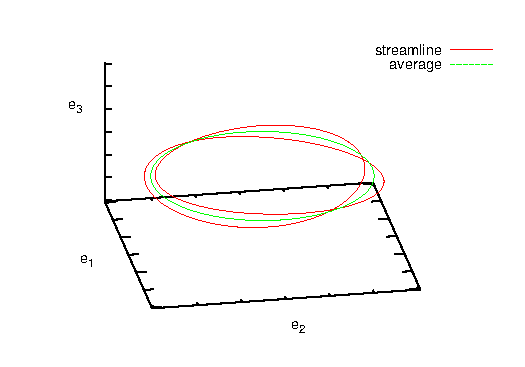
\includegraphics{trefoil_knot.pdf}
% %  \caption{
% %    A possible streamline (red) with its averaged rotation in green.
% %    The streamline was chosen to be a trefoil knot. The reasons for the non-trivial topology are discussed in the text.
% %    }
% %    \label{fig:particle}
% % \end{figure}



% \section{The force law for a turbulent  source}\label{sec:int:vortex_interaction}
% The force law for an acoustic source when in the presence of an external vorticity or Coriolis field may be found 
% from the manifestly gauge invariant energy momentum tensor\cite{Doran2003}, equation \eqnref{TAEM}.
% Remembering Maxwell's relation, $\del\cdot F = J$ (equation \eqnref{Maxwell})
% we obtain 
% \begin{align}
%  f = \scope T(\scope \del) = -\half \lr{\scope F\scope \del F + F \del F} = -\half \lr{-JF +FJ} = J \cdot F.
% \end{align}
% If the acoustic source has a constant rest mass, $m_0$ and moves at a speed $u$,
% then, by writing  $J = q u$, where $q$ is the acoustic source, we obtain
% \begin{align}
%   f = m_0 \dot u = q u \cdot F, \label{eqn:LFL}
% \end{align}
% Equation \eqnref{LFL}  is the Lorentz force law.

% To write equation \eqnref{LFL} in its more conventional form we project into the laboratory frame,
% \begin{align}
% J\cdot F  = \scalar{\lr{\rho + \vJ} \g\lr{\vE+I\vB}} = -\lr{J\cdot E + q \vE + q \vu\times\vB }\g.
% \end{align}
% The timelike $q\vu\cdot\vE $ is the work done.
% The remaining spatial component is
% \begin{align}
%    \vf = -q \lr{\vE + \vu \times \vB},
% \end{align}
% which is the Lorentz force law in its usual form.

% Equation \eqnref{LFL} describes how a turbulent source moves 
% in the presence of external flows when measured with ultrasound.
% Its linearity is an example of the general rule that the world appears more simple
% when it is measured acoustically.
% This is because, due to the limitations on what ultrasound can measure, reassigns the temporal and spatial locations of entities so that 
% the non-linearity in their motion vanishes.

% % The divergence of the energy momentum tensor gives the force
% % and the spatial component in the lab frame is
% % \begin{align}
% %   \vf = - \lr{\rho_q\vE + \vJ \times \vB}.
% % \end{align}
% % If it is assumed that an acoustic charge $q$ is carried by a `particle' moving at speed $\vu$, then
% % $\vf = - q\lr{\vE + \vu \times \vB}$, which is the Lorentz force law.
% % Turbulent sources of sound, therefore, interact according to the Lorentz-force law when measured acoustically.

% %\subsection{Particles with Spin}

% \section{Further work: Interactions between particles with spin}\label{sec:int:electron}

% The (exact) analogy developed in this thesis between acoustics and electromagnetism
% is incomplete in that we are missing an analogue to the electron:
% a particle with spin that  interacts with the spin of the sound pulse.
% We have found that turbulance is the source of the sound
% field - a role played by the electron for electromagnetic waves - 
% but we have not found an analogy of the electron itself.
% %Here we suggest path  for completing the  analogy.
% %We hope that it will  provide be a useful start to future research.

% In \secref{} we found that the spin parallel to the momentum 
% can be interpreted as resulting from  helical trajectories of the fluid particles through spacetime,
% with the spin resulting from the  orbital angular momentum of the fluid precession  about a mean trajectory.
% For this helicity not to integrate to zero,
% Moffatt demonstrated that the trajectory of the fluid particles must be knotted in some manner.
% The acoustic electron is presumably, therefore, comprised of a confined region of fluid undergoing some form of knotted helical motion.


% Interpreting the electron's trajectory as a helix about a mean trajectory is not a new idea. 
% It is at the core of the \zitter\ interpretation of quantum mechanics which dates back to Schr\"odinger.
% It has more recently overhauled by David Hestenes, and put into a form consistent with the Dirac equation\cite{}.
% In the \zitter\ interpretation the spin of the electron is interpreted as the orbital angular momentum of the electron 
% about its centre path.

% %
% %and provides the most promising starting point for our analogy.
% Using the \zitter\ as our starting point,
% we identify the electron with a region of the fluid undergoing helical motion.
% We do not assume that the actual fluid particles within the region are fixed,
% a given particle may flow through the region.
% We then use consistency with the Dirac equation to impose constraints upon this trajectory.
% As might be expected, the constraints are stringent and we are unable imagine how such a streamline can arise
% in acoustics.
% Nevertheless,
% it does give a beginning on which to build.

% \subsection{Correspondence with the \zitter\ model}

% The requirements for \zitter\ to be consistent with the Dirac equation have been catalogued.
% Here we discuss the list given in David Hestenes' article on self-interaction\cite{},
% \nlist{
%   \item the acoustic electron is a massless point particle. \label{index:massless}
%   \item the orbital-angular momentum, or spin, about the helix is fixed at $s=\hbar/2$, \label{index:spin}
%   \item the frequency of the precession is the de Broglie frequency $\omega_0 = mc^2/\hbar$,\label{index:freq}
%   \item the acoustic electron has a charge $e$
%   \item the total energy of the acoustic electron is $mc^2 = E_0 + U_0$ where $E_0$ is the kinetic energy of the helical trajectory,
%     and $U_0$ is the self-interaction potential.
% }
% From property \ref{index:massless} it follows that the helical trajectory travels at the speed of sound.
% This is not to say that the acoustic-electron travels at the speed of sound, 
% however, 
% for the projection onto the mean path will be timelike.
% From property \ref{spin} we find that the spin of the acoustic wave is constrained to be half that of the sound pulse.

% The radius of the helix is (from \ref{index:freq}) 
% \begin{align}
%   r = \frac{c}{\omega} = \frac{\hbar}{mc}
% \end{align}
% From property \ref{index:spin} it follows that
% %\begin{align}
%   $s = r\frac{E_0}{c} = \frac{\hbar}{2}$
% %\end{align}
% and so 
% \begin{align}
%   E_0 = s \omega_0 = mc^2/2
% \end{align}
% from which it follows that $E_0 = U_0 =  mc^2/2$.

% The magnetic moment - or vorticity moment - 
% is 
% \begin{align}
% \mu = \frac{ec}{2\pi r}\frac{\pi r^2}{c} = \frac{er}{2} = \frac{e}{mc}s = \frac{e\hbar}{2mc}
% \end{align}

% The Dirac current is then interpreted as the most probable mean trajectory 
% and the spin current is interpreted as the most likely direction of the spin at each spacetime point.

% \subsection{Discussion}


% To pursue the analogy between the electron and acoustics we need an algebraic system that unifies as much as possible
% classical and quantum physics.
% David Hestenes geometric algebra does this very elegantly.
% As has been forcefully demonstrated by Hestenes\cite{HestenesMechanicsBook} 
% and Doran and Lasenby\cite{Doran2003},
% much of the `quantum mathematics' has nothing intrinsically tied to quantum mechanics, 
% but rather describes mechanics in a 4-dimensional spacetime.

% Using this algebraic system
% we find that many of the features that we wish to 
% incorperate into the vortex-with-helicy-sound interaction are already present 
% in David Hestenes Zitterberegung model of the electron,
% which we use as a template.
% The  Bjerknes model of pulsations suggests an interpretation to the 
% electron's interaction parameter $\beta$, 
% which is the only parameter without adequate interpretation in the Dirac-Hestenes model.

% While the analogy between a pulsating bubble and an electron is far from satisfactory,
% it is true to say that a pulsating bubble has most of the ingredients required.
% It therefore makes an interesting first attempt, and a good point of departure for further research.





% Vortex rings with swirl,
% by virtue of their angular momentum about their symmetry axis, have been used as  classical models of spin \cite{Pekeris1953}.
% It is, however, the link between topology, helicity and spin that makes the analogy more than a useful conceptual aid.
% Moffatt \cite{Moffatt1969}, for example, when considering Hicks' spherical vortex notes  that 
% ``every torus knot is represented once and only once amongst all the vortex lines of each member of the family of flows described by the stream function''.
% Accordingly, the intrinsic angular momentum of such toroids 
% can be at least partially identified with its spin.
% %The spin will interact with an external vorticity field with a magnetic moment type reaction.
% %By appeal to the electromagnetic analogy we call the strength of the interaction the {\em magnetic moment}.
% %Since there is no danger of confusion, it seems better to use the terms of the analogy rather than introducing names such as {\em vorticity-moment}.
% %The magnetic moment is $\mu = \gamma_g \vs$ where $\vs$ is the spin vector and $\gamma_g$ is the giromagnetic ratio.
% %The energy of the interaction is $H = \mu \cdot \vB$. % and accordingly the force is $-\vdel H =-\vdel  \mu\cdot \vB$.
% %The spin-vorticity interactions need to be added
% %to the Lorentz force law of \eqnref{LorentzGA}.


% The kinematics of a vortex ring can be modelled by placing a local orthonormal coordinate frame $\{e_0, e_1, e_2, e_3\}$ at the centre of the ring.
% The vector $e_0$ is timelike and is tangent to spacetime path of the centre of the vortex, $x(\tau)$.
% Then, with $\tau$ being the proper time, $e_0 = \frac{dx}{d\tau} = u$, where $u$ is the velocity, and $e_0^2 = 1$.
% The three orthogonal axes are spacelike, so that $e_i^2 = -1,$ for $i = 1,2,3$.
% The vector $e_3 = s$ is oriented so that it is  orthogonal to the vortex ring, and is called the spin vector.
% The vectors, $e_2$ and $e_1$ define the {\em spin-plain}, $S = e_2e_1$ on which the vortex ring is confined.
% The vector $e_2$ is set to point towards the average motion of a particular swirling particle (following the green line in  \figref{particle})
% enabling the magnitude of the spin to be captured.

% %If the vortex is moving inertially, its momentum $p$ will be constant.
% %%$m$ is a measure of the vortex's intrinsic mass, perhaps the mass difference displaced by any pressure gradients within the vortex.
% %By defining and effective mass, $m =  p \cdot u$ and integrating, it follows that  $p\cdot(z - z_0) = m\tau$.
% %If the angular momentum is conserved then $lr{z - z_0} \wedge p = S(\tau) - S_0$ and so the equation of motion follows
% %\begin{align}
% %z = (S(\tau) - S_0) \cdot p^{-1} + m p^{-1} \tau + z_0 = x(\tau) + r(\tau),
% %\end{align}
% %where $x(\tau) = S_0 \cdot p^{-1} + m p^{-1} \tau + z_0 $ is the spacetime path of the central line, 
% %and $r(\tau) = S(\tau)  \cdot p^{-1}$ is the radius of the vortex ring.
% %The particle that is followed by $e_2$ is then seen to follow a helix of radius $r$ in spacetime.
% Although it is not immediately obvious,
% the model presented so far is essentially identical to the `timelike' case of the David Hestenes zitterbewegung interpretation of 
% electron physics 
% \cite{Hestenes1973, Hestenes1990,  HestenesResearchProgram}. 
% We apply the results of these papers freely, 
% although argue the results in terms of the meaning to acoustically measured turbulence. 


% The motion of the reference frame $\{e_\mu\}$ models the motion of the vortex
% and can be obtained from a constant reference frame, $\{\gamma_\mu\}$ by means a Lorentz rotation.
% Rotations are double sided transformations in geometric algebra, 
% and is written,
% $e_\mu = R \gamma_\mu \Rt$,
% where the {\em rotor} $R$ is an even multivector with reverse $\Rt$, such that $ R\Rt = 1$.
% Since geometric positioning of $\{e_\mu\}$ is all that is modelled,
% the kinematics of the frame can be completely determined by finding the
% $\tau$-dependent bivector $\Omega =  2\dot{R}\Rt $, which represents the angular
% velocity of the frame,
% %kinematics is expressed entirely by the rotor $R$,
% %such that
% %\eqal{
% %\dot{R} = \half\Omega R.
% %}{RotorEqn}
% %Alternatively, the influence on each axi
% \begin{align}
%   \dot e_\mu = \Omega \cdot e_\mu
% \end{align}
% The Lorentz force in \eqnref{LorentzGA} is of this type, with $\OmegaEM = \frac{q}{m_0}F$.
% %where $\Omega =  2\dot{R}\Rt $ is an 
% %The dynamics of the frame can be completely determined by finding the
% %$\tau$-dependent bivector $\Omega =  2\dot{R}\Rt $, which represents the angular
% %velocity of the frame.

% The energy of the fluid in the vortex is modelled by the rotation of $e_2$ in the spin plain $S$.
% Therefore, energy-momentum of the vortex is described by the rotation in this plain, $\Omega \cdot S$.
% %The quantisation of the spin in \secref{lagrangian} came from the knottedness of the flow around the spin-plain, 
% %which implies that $\oint \lr{ dx^\mu \Omega_\mu} \cdot S = nk$,
% %where $k$ is the vortex strength and $\Omega_\mu$ is the acceleration in the direction of $\gamma_\mu$.
% To include interactions with sound wave, 
% %If the vortex interacts with sound then for the angular momentum to be both conserved and obey the quantisation,
% it should be the  {\em canonical energy-momentum}, $P = p - eA$, that is equated to $\Omega \cdot S$.
% %It is appropriate that the sound contributes its energy to the spin, 
% %for this is the only way in which angular momentum is conserved. 
% Therefore
% \begin{align}
%   \Omega\cdot S = P \cdot u = m - eA\cdot v.
% \end{align}
% If a sound wave deposits $\OmegaEM \cdot S$ of energy to the vortex ring, then its mass must also increase.
% %The  $m = p \cdot u$ cannot therefore be equal to the free vortex mass $m_0$,
% %but must be
% Therefore
% \begin{align}
%   m  = p \cdot u =  \Omega \cdot S + eA\cdot v= m_0 + \OmegaEM \cdot S + eA\cdot v.
% \end{align}
% The other components of the angular velocity in the direction orthogonal to the spin plain is labelled $ v\cdot  ( I q) =- v\cdot (\Omega \wedge S)$
% while the rate at which the spin plain changes direction as it moves round its axis is $\dot S = v \cdot \del S = \Omega \times S$.
% Note that the symbol $\times$ here represents the commutator product rather than the Gibbs vector product.
% Bringing all the components together
% \begin{align}
% \label{eqn:OmegaS}
% \Omega S = \Omega \cdot S + \Omega \times S + \Omega \wedge S  = v \cdot P + \dot S + Iq
% \end{align}

% An explicit expression for $\Omega$ can be obtained by setting
% \begin{align}
%   \label{eqn:OmegaS2}
%   \Omega S &= m_0 + \OmegaEM S && \implies & \Omega &= m_0 S^{-1} + \OmegaEM = m_0 S^{-1} + \frac{e}{m_0} F.
% \end{align}
% Clearly then \eqnref{LorentzGA} is satisfied.
% Also it follows that  $\dot S = \frac{e}{m_0} F \times S$ which gives an expression for the precession of the spin plain due to the magnetic moment.

% Combining \eqnref{OmegaS} and \eqnref{OmegaS2} gives
% \begin{align}
%    v \cdot p- eA\cdot v  + v \cdot \del  S - v\cdot  (I q)=m_0 + \frac{e}{m_0} F S = m - eA\cdot v 
% \end{align}
% This is the classical approximation  of the Dirac equation in the absence of statistical terms \cite{Hestenes1990}.
% The full  equation in the absence of statistical terms is 
% \begin{align}
%  p -Iq +  = mv - \del S.
% \end{align}
% The similarities and differences  between these equations is found in the literature \cite{Hestenes1990}.


% A simple example of bound hydrodynamic helicity is Hick's spherical vortex\cite{Moffet1980}.
% This model is particularly interesting to us for it also 
% models the flow of a gas within a large bubble, where the surface tension can be neglected.
% Pulsations can futher be incorperated in an elementary way by 
% adapting the technique of Carl and Vilhelm Bjerknes to separate the interaction term caused by the pulsation 
% from the underlying force law.
% A second virtue of Hick's votex is that the angular momentum is conserved when the speed of sound is
% equal to the speed of light, which is exactly our measurement condition.
% Indeed, Pekerisis found that this conservation law applies {\em only} when the sound speed equals the speed of light.
% Pekerisis had no physical reason to impose this condition on the world, 
% but nevertheless considered the possibility of using Hick's vortex to model a neutron.
% %With the conditions of acoustic measurement considered in \chapref{measurement},
% %such a calculation seems entirely natural.
% \section{Modelling an oscillating Bubble}\label{sec:bubble}
% %Micron-sized bubbles are resonant at medical ultrasound frequencies and are used as contrast agents
% %for they  greatly enhance the signal  from blood which is generally echo-poor.
% %To consider their acoustic output it is often sufficient to ignore turbulence and simply calculate the oscillations of a monopole source.
% %However, their {\em motion} will generally not be free from turbulence effect - indeed, the microbubbles are often used to {\em measure} such turbulence.
% %It would be nice to bring their interactions with sound into the general framework presented so far.
% %To do so, the bubble is assumed to be an enclosed vortex. 
% %Toroidal bubbles bound in a region of vorticity have been observed many times - and even generated by Dolphin's in play \cite{}.
% %A spherical vortex with swirl is stable even when stationary in the fluid - and it is this flow that we imagine within a bubble.
% %In the model presented, the mass of the vortex increases when it absorbs a sound wave.
% %This models the volume fluctuations only at their most crude,
% %although for the purpose of dynamics this may be sufficient.


% To adequately model the dynamics of pulsating body such as a bubble, the  {\em interaction parameter}, $\beta$  needs to be introduced into the model.
% This can be done by substituting  $F \rightarrow F e^{I\beta}$ in the model above.
% Since the bubbles are very small, we additionally introduce a probability density $\rho$ for their location 
% - where the symbol $\rho$ should not be confused with the mass or charge density.
% Inserting these into the model above results in
% \begin{align}
%    \rho v \cdot p e^{-I\beta}  + v \cdot \del  \lr{\rho S e^{I\beta}} - \rho v\cdot  (I q)= \rho m \cos\lr{\beta}
% \end{align}
% This is the classical limit to the full Dirac equation including `statistical factors' \cite{Hestenes1973}
% The interaction intensity $\beta$ is uninterpreted in Dirac theory, although it is known to be important for determining whether an election is in a particle or anti-particle state.
% Here $\beta$ plays a similar role (it determines whether the force is attractive or repulsive).
% Whether the identification stands up to scrutiny remains to be seen.
% \section{The acoustic analogy to the electron}\label{sec:int:electron}


% %The derivation is most convenient when using David Hestenes geometric algebra\cite{} and will be used here.
% %This is because only in this algebra can Maxwell's relations be expressed in a single equation.
% %Furthermore, the vector notation of Geometric algebra should be familiar even to non-afficienardos,
% %and so its use should not be a hinderence to meaning.


% Acoustic sources will, in general, interact with one another. %, with this interaction  mediated by sound.
% %The study of vortex-vortex interactions has a  long history  \cite{Whittaker1951},
% The study of the interactions between pulsating bodies
% is of  interest in medical ultrasound because pulsating micron sized bubbles are used as contrast agents.
% The induced motion  between neighbouring bubbles has been photographed
% and the force between them is often  modelled according to Bjerknes' law  \cite{Crum1971}.
% This states that the average force on a bubble, $\scalar{f}$, is
% equal to volume displaced by the bubble, $ V$, multiplied the acceleration 
% induced by a pressure gradient, $\vdel p$ \cite{Bjerknes1905,Crum1971, Leighton1990},
% \begin{align}
%   \label{eqn:Bjerknes}
%   \scalar{f} = \scalar{V(t)\vdel p(\vx, t)}.
% \end{align}
% The  average force  over an oscillation cycle will not be zero if the bubble do not pulsate in phase with the sound wave.
% % f the oscillations arThe phase is denoted with a 
% % % and the pressure oscillates sinusoidally with a frequency $\omega$, so that  $P(\vx, t) = P(\vx)\sin\lr{\omega t}$.
% % To see that the average can give non-zero results,
% If we assume that the spatial and temporal components of the pressure may be separated, 
%  so that  $P(\vx, t) = P(\vx)\sin\lr{\omega t}$,
%  and assume that the bubble's pulsations are small, 
%  so that $V(t) = V_0\sin\lr{\omega t + \beta}$,
% then 
% $\beta$ is the phase of the bubble's oscillations in comparison to the driving sound wave.
% %Then 
% %\begin{align}
% %  \scalar{F} = V_0\vdel P(\vx) \scalar{\sin(\omega t+\beta)\sin(\omega t)} =  \frac{1}{2}V_0\vdel P(\vx) \cos(\beta)
% %\end{align}
% The resultant force over a cycle of oscillation is 
%  $\scalar{F} = \frac{1}{2}V_0\vdel P(\vx) \cos(\beta)$.
% %The strength of the force is determined by $\cos(\beta)$,
% %which can be either positive or negative.

% The  cost of this simple model is that the equations describing the surrounding fluid are linearised.
% Vorticity is not considered and we are entirely removed from the general problem of 
% turbulence-sound interaction.
% This is a shame, for while it is true that the acoustic output of a pulsating bubble far exceeds that of turbulent sources,
% turbulence is still excepted to have an influence on the bubble's motion.
% %Bubbles will not only be carried by turbulent flow but will also interact with the sound generated by it.

% Bjerknes' law, in itself, assumes little about the bubble. 
% It requires only a pulsating volume.
% The details of the bubble, such as its surface tension, are hidden in the parameter $\beta$ that specifies how close to resonance the bubble is \cite{Leighton1990}.
% The motion and interaction of a bubble, therefore, 
% can be firmly set within the context of turbulence-sound interactions, 
% so long as the bubbles mass varies when the bubble interacts with an acoustic field.
% This chimes with the attempts to use Hicks'  spherical vortex as a model of a bubble \cite{Levine1959}.
% Indeed, so long as the bubble is small compared 
% to the wavelength of the sound with which it interacts, then any vortex should do.
% %Bjerknes' law not require us to be too specific.


% In this report, as a means of investigating the interactions between bubbles and sound in its full context,
% models to describe sound-turbulence interactions in general are suggested.
% To simplify the approach we consider only the special case of when the interactions are measured acoustically,
% such as is the case when the turbulence is measured with ultrasound.
% %The formulation therefore remains general, 
% It turns out that  acoustics  is greatly simplified when imaged with sound.
% In fact,
% as is shown in \secref{measurement},
%  Lighthill's formulation of acoustics reduces to an {\em exact} analogue of electromagnetism.
% The reasons for this are briefly discussed in \secref{measurement} 
% and in more detail in a companion paper elsewhere in these proceedings.

% To find the physical consequences of the equivalence,
% the analogy is used to define an acoustic Lagrangian.
% %The exactness of the analogy has a number of consequences.
% %To find them, it is noted that since the field equations are the same, 
% %the acoustic field and the electromagnetic field 
% %can be characterised by a common Lagrangian.
% This is done in \secref{lagrangian} and the implications to angular momentum and helicity are discussed.

% Starting from the Lagrangian, the acoustic energy momentum tensor follows,
% from which the required interaction laws between sound and turbulence can be found.
% Unsurprisingly, in light of the analogy found, 
% this is the Lorentz force law  (\secref{spinless}).

% Swirl, which is  the motion along a vortex ring, for example, is harder to incorporate.
% This is because, as argued in \secref{spin}, a vortex with swirl has an intrinsic angular momentum
% which will be involved in the interaction.
% To simplify, the size of the vortex is reduced to a point.
% Its swirl and velocity can then be modelled with a co-moving frame of reference,
% %One axis of the coordinate frame traces the path of the vortex,
% %another traces the rotion.
% %The helical path through spacetime of any given particle within the vortex can then be traced.
% %This is discussed in \secref{spin}.  
% The interaction term $\beta$ is included in \secref{bubble},  enabling bubble motion to be modelled.
% The model chosen has a great deal of common with classical models of quantum  spin.
% Our thinking has been particularly influenced by David Hestenes' timelike  Zitterbegung model of the election \cite{Hestenes1973, Hestenes1990, HestenesResearchProgram}.  
% It is interesting how naturally the zitterbewegung model can be applied to turbulence.

% Finally, we note that the geometric nature of the models discussed is most straightforward
% and  concise when expressed in the {\em Spacetime Algebra} of David Hestenes \cite{Hestenes2003}.
% %This notation is sufficiently close to usual 3-dimensional vector algebra to be familiar,
% %but unfortunately space here does not permit an introduction to the algebra.
% Important results will be projected into the laboratory frame,
% so that they can be understood entirely with familiar 3-dimensional vector algebra.
% We use the convention that three dimensional vectors are displayed in bold.
% This helps to distinguish them from their spacetime analogues.

% \section{Discussion}\label{sec:discussion}

% We have constructed a general model for the dynamic interactions between sound, turbulence and bubbles.
% If the model is confirmed experimentally,
% then it represent a  relatively simple yet powerful framework in which to investigate the motion and dynamics of acoustic sources.

% In order to be able to construct the models the following observations were necessary:
% \nlist{
% \item  That the measurement process used in acoustical measurement is identical to that used in optical relativistic theories,
%     but with the speed of sound taking the role of the speed of light.
% \item  That acoustics formulated on an incompressible, relativistic ideal fluid (which embodies measurement considerations)
%     is identical to classical electromagnetism.
% }
% The authors are unaware of these observations having been made before.

% Having made the link between electromagnetism and acoustics, 
% for which a relativistic theory is  a pre-requisite,
% the application to acoustic interactions followed more-or-less mechanically.
% This indicates, on the one hand, the potential power of the analogy.
% It represents, on the other hand, a set of stringent experimental test with which to test the link between acoustics, relativity and electromagnetism.



% \section{Discussion}



% %%%%%%%%DISCUSSION
% The correspondance is exact, and successfully unifies the much observed the similarites
% between the magnetic field and vorticity (which was used by Maxwell)
% and the electric field and the corriolis acceleration (\cite{Marmanis2000,Sridar1998})
% Marmanis\cite{Marmanis} and Sridar\cite{1998} analogies were only partial 
% due to their application of the Gallilean invariance rather than
% the Lorentz invariance appropiate for electromagnetism and ultrasound.
% %%%%%%%%%%%%




% We have shown that Maxwell's equations may be derived from a relativistic (Lorentz invarient) ideal fluid,
% where the speed of sound takes the role of the speed of light.
% The Coriolis acceleration - also known as the Lamb vector - takes the role of the electric field 
% and that the vorticity takes the role of the magnetic field.
% The relativistic vorticity bivector takes the role of the field tensor.
% This identification of terms was made before by Mermanis\cite{Mermanis}.
% However, their attempt started from the Gallilean invarient approximation 
% and so Maxwell's equations could not be written down while still maintaining sound as the propergating medium.
% This work completes their analogy by making it exact.

% At first, however, the analogy derived here is dissapointing.
% A relativistic fluid, where the speed of sound equals the speed of light, 
% seems so esoteric that applications for the analogy seem in short surply.
% There is a major and terrestial application for the analogy, however,
% and that is to ultrasound physics.

% In ultrasound distances are determined from 
% \nlist{
% \item the time interval between a sound pulse leaving the transducer
% and the echo returning,   
% \item the average speed of sound of the medium.
% }
% The average speed of sound of the medium is required before anything can be said about the locations of entities
% in the world.




%%% Local Variables: 
%%% mode: latex
%%% TeX-master: "tshorrock_thesis"
%%% End: 

% LocalWords:  helicity aeroacoustics
